\documentclass[../TST.tex]{subfiles}
\begin{document}
\begin{eproblem}[Measuring the refractive index of a liquid]{\ \\[5pt]}
\textit{Equipment:}\\
Plastic petri dish (shallow cylindrical dish for cell culture use), unknown liquid, pins, piece of corrugated cardboard, ruler, graph paper, pens (3 colours). See Figure \ref{fig2}.
\begin{figure}[h]
\centering
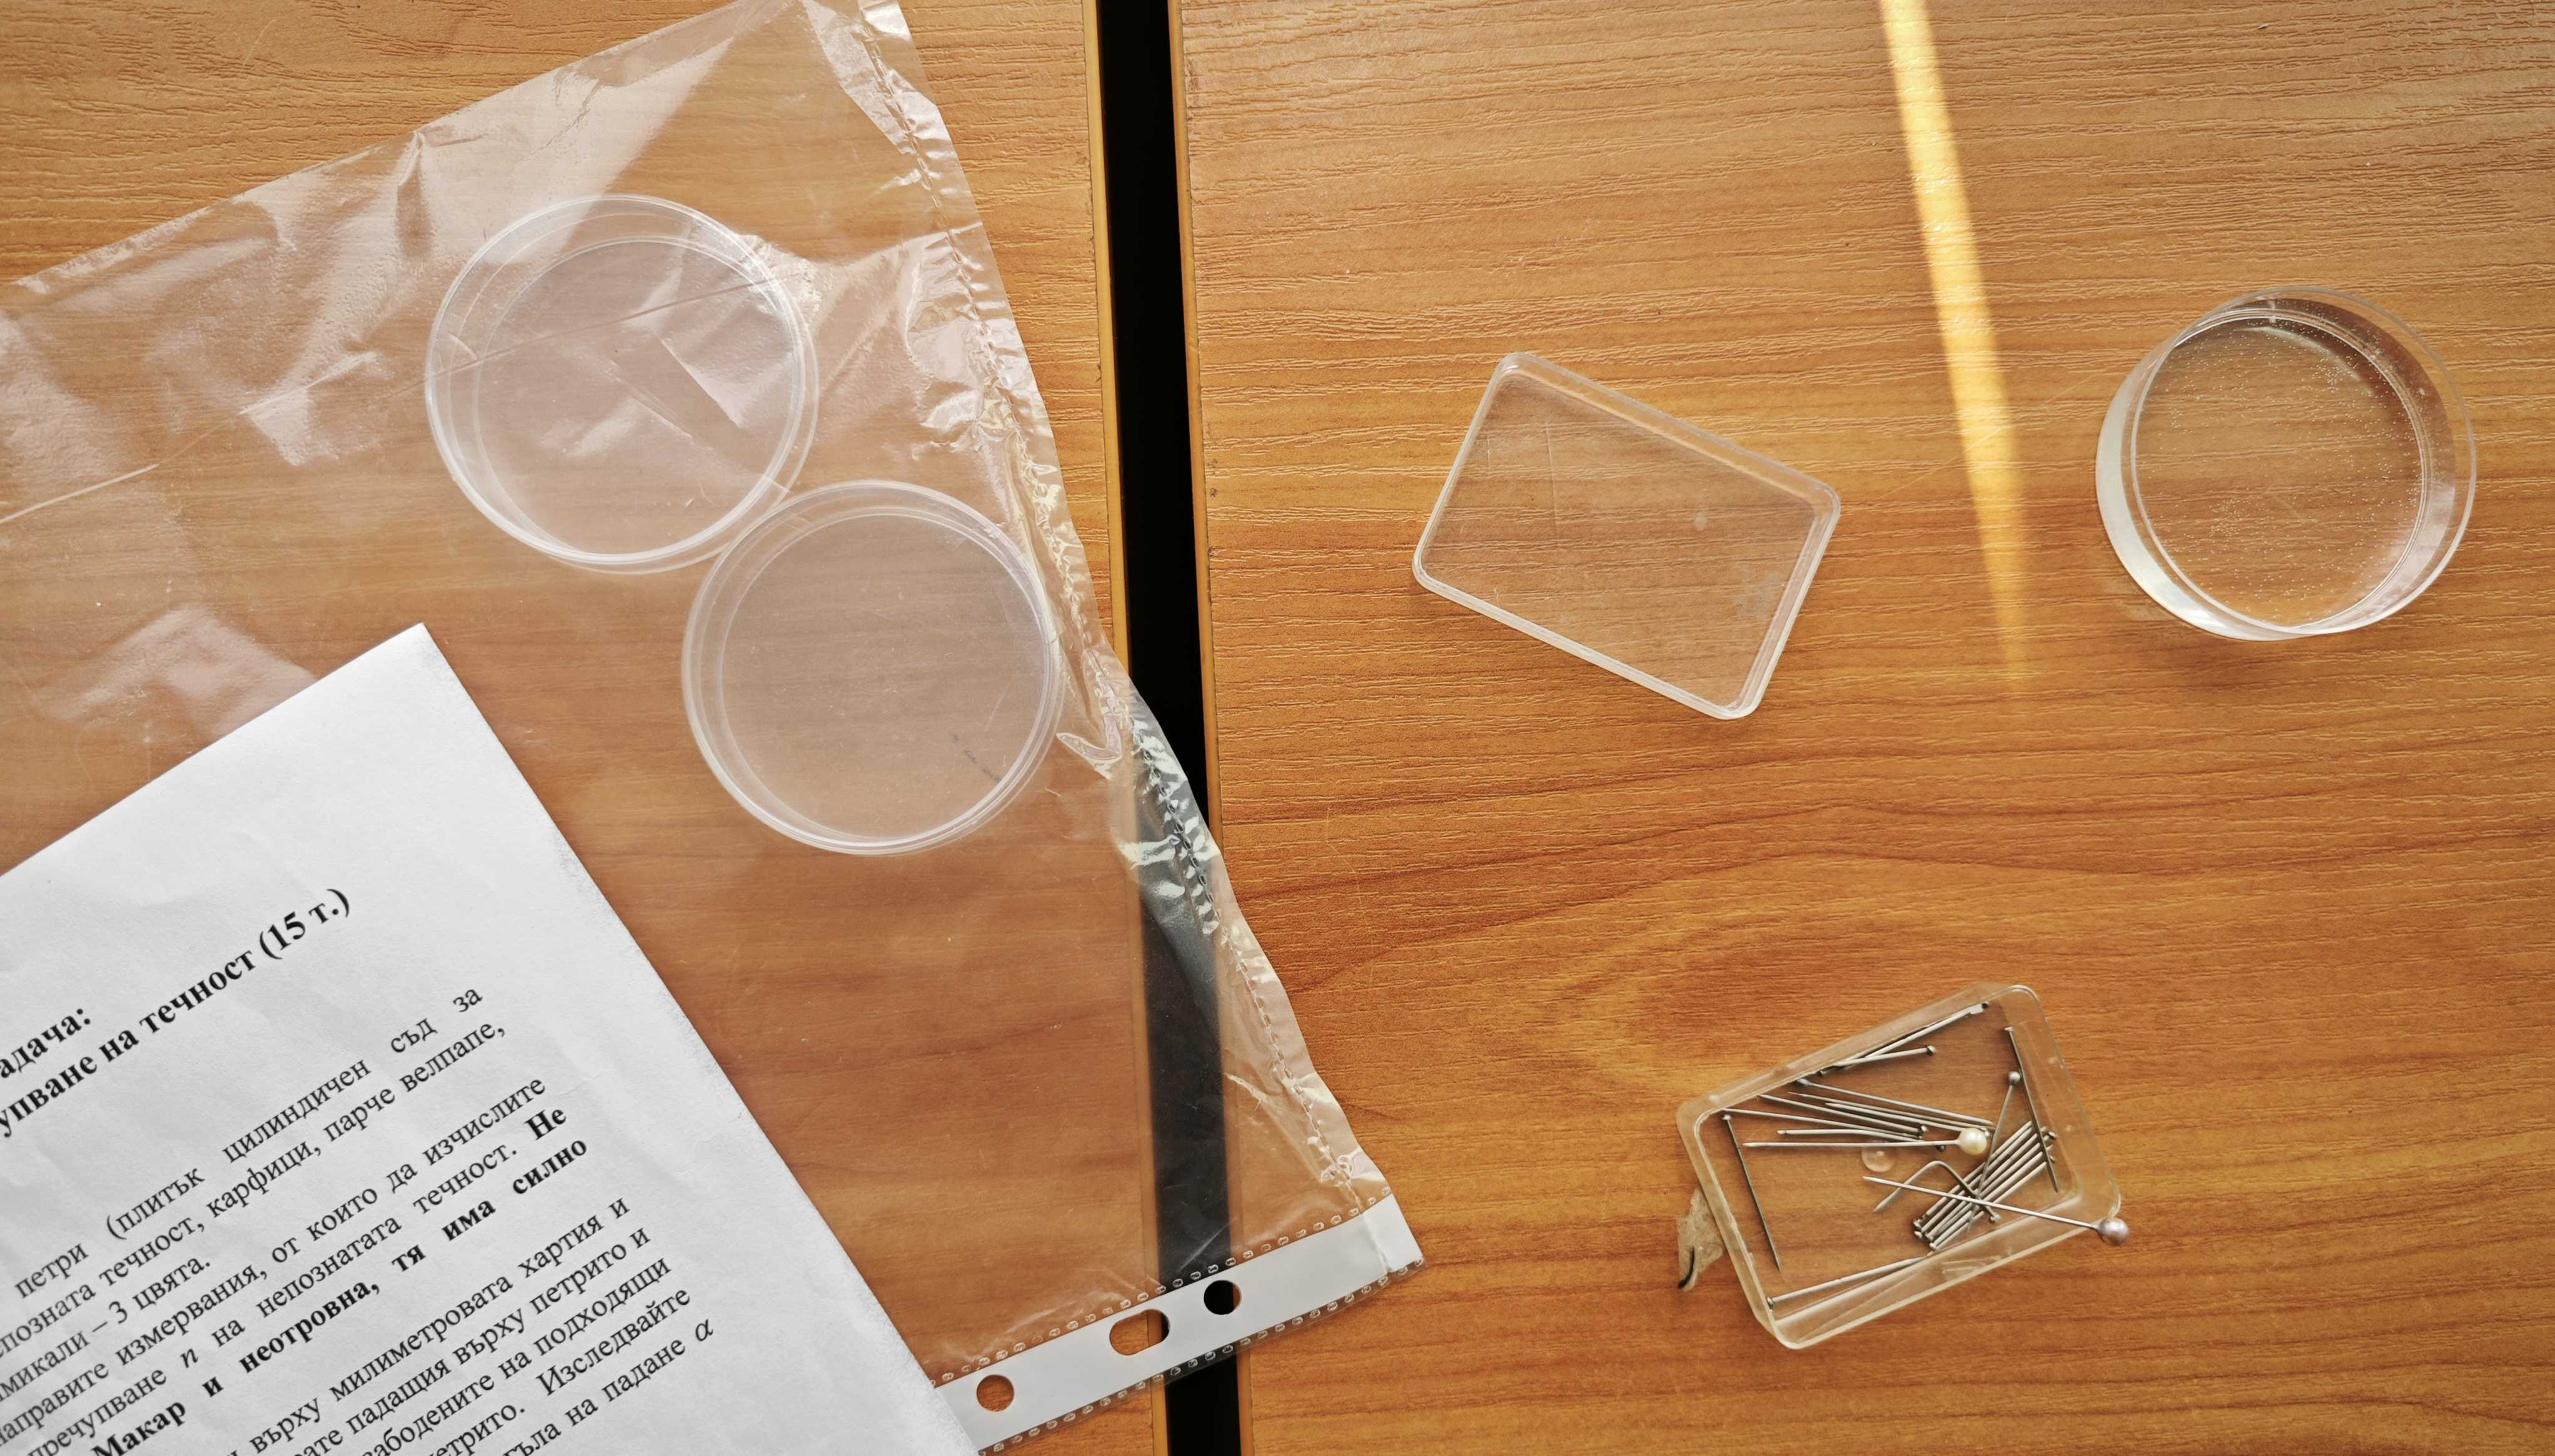
\includegraphics[width=0.6\textwidth]{fig/2012_e1.jpg}
\caption{}
\label{fig2}
\end{figure}

The aim of this problem is to find the refractive index of an unknown liquid through the appropriate measurements. Do not taste the liquid! Though non-toxic, it has strong laxative properties\footnote{This turned out to be a lie, as the liquid was just a sugar solution.}!\\[5pt]
Fill the the petri dish with the liquid and place it on top of the graph paper and the corrugated cardboard. Use the pins to mark the incident and the outgoing rays. Observe the images of the pins through the side of the petri dish. Study the dependence of the angle of deviation $\varphi$ on the angle of incidence $\alpha$ (Figure 2). These angles are related by

\begin{equation*}
	\sin{\alpha}=n\sin{\left(\alpha - \frac{\varphi}{2} \right)}
.
\end{equation*}
Assume that the plastic has the same refractive index as the liquid.
\begin{figure}[h]
\centering
\hspace*{0.6cm}
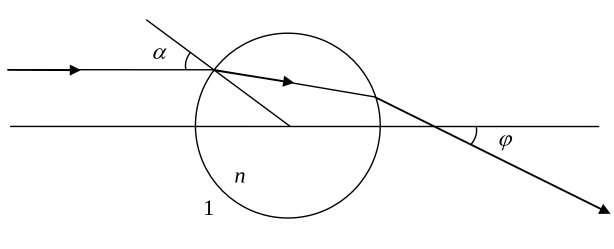
\includegraphics[width=0.6\textwidth]{fig/2012_e2.png}
\caption{}
\label{fig3}
\end{figure}

\begin{subpart}
	\item State the parameters that you will be measuring. Take enough useful measurements. Present them in a table and explain how they were obtained. \score{6.0} 
	\item State the variables which, when plotted, can easily give you $n$. \score{0.5}
	\item Plot the relevant graph. \score{4.5}
	\item Using the graph, determine the refractive index $n$. \score{3.0}
	\item Estimate your error in finding $n$. \score{1.0}
\end{subpart}
Call the examiner in case of any technical difficulties.\\
\end{eproblem}
\end{document}
